\newpage

\lecture{13}{9 Dec. 13:20}{}

\section{Diagonalization of a Matrix}

\begin{definition}
    An $n\times n$ matrix $A$ is said to be \textbf{diagonalizable} if there exists a nonsingular matrix $S$ such that \[
        S^{-1}AS = \Lambda
    \]
    where $\Lambda$ is a diagonal matrix.
\end{definition}

\begin{theorem}[5C]
    Suppose $A_{n \times n}$ has $n$ linearly independent eigenvectors $x_1, x_2, \ldots, x_n$. Let $S$ be the $n \times n$ matrix with $x_1, x_2, \ldots, x_n$ as its columns. Then \[
        S^{-1}AS = \Lambda = \begin{pmatrix}
            \lambda_1 & 0 & \cdots & 0 \\
            0 & \lambda_2 & \cdots & 0 \\
            \vdots & \vdots & \ddots & \vdots \\
            0 & 0 & \cdots & \lambda_n
        \end{pmatrix}
    \]
    where $\lambda_i$'s satisfy $Ax_i = \lambda_i x_i$.
\end{theorem}
\begin{proof}
    Suppose $S = (x_1 \mid \cdots \mid x_n)_{n \times n}$. Then \begin{align*}
        AS &= (Ax_1 \mid \cdots \mid Ax_n) = (\lambda_1 x_1 \mid \cdots \mid \lambda_n x_n)_{n\times n}\\[6pt]
        &= (x_1 \mid \cdots \mid x_n) \begin{pmatrix}
            \lambda_1 & 0 & \cdots & 0 \\
            0 & \lambda_2 & \cdots & 0 \\
            \vdots & \vdots & \ddots & \vdots \\
            0 & 0 & \cdots & \lambda_n
        \end{pmatrix} = S\Lambda
    \end{align*}
    \[
        \implies S^{-1}AS = \Lambda
    \]
    for nonsingular $S$.
\end{proof}

\begin{remark}[1]
    If $\lambda_1, \ldots, \lambda_n$ are distinct, then the eigenvectors $x_1, \ldots, x_n$ are linearly independent. In other words, a matrix with distinct eigenvalues can be \blue{diagonalized}.
\end{remark}

\begin{remark}[2]
    The diagnoalizing matrix $S$ is \red{not} unique. Repeated eigenvalues leave more e.g.
    \[
        S^{-1}IS = I 
    \]
    is true for any nonsingular $S$.
\end{remark}

\begin{remark}[3]
    $AS = S\Lambda$ holds if and only if the columns of $S$ are eigenvectors of $A$.
\end{remark}

\begin{remark}[4]
    Note all matrices posses $n$ linearly independent eigenvectors and therefore not all matrices are diagonalizable.
\end{remark}

\begin{theorem}[5D]
    The eigenvectors $x_1, \ldots, x_n$ coorsponding to the distinct eigenvalues $\lambda_1, \ldots, \lambda_k$ of $A$ are linearly independent.
\end{theorem}

\begin{eg}
    \[
        \begin{pmatrix}
            1 & -1 \\
            0 & 1
        \end{pmatrix}
    \] where $\lambda_1 = \lambda_2 = 1$ 
\end{eg}
\[
    \begin{pmatrix}
        1 & -1 \\
        0 & 1
    \end{pmatrix} \begin{pmatrix}
        x_1 \\ x_2
    \end{pmatrix} = \begin{pmatrix}
        x_1 - x_2 \\ x_2
    \end{pmatrix} \quad \implies \quad x = \begin{pmatrix}
        x_1 \\ x_2
    \end{pmatrix} = t \begin{pmatrix}
        1 \\ 0
    \end{pmatrix},\ t \in \mathbb{R}
\]

Let $P = \begin{pmatrix}
    1 & 2 \\
    0 & 0
\end{pmatrix}$, when we have
\[
    AP = \begin{pmatrix}
        1 & -1 \\
        0 & 1
    \end{pmatrix} \begin{pmatrix}
        1 & 2 \\
        0 & 0
    \end{pmatrix} = \begin{pmatrix}
        1 & 2 \\
        0 & 0
    \end{pmatrix} \begin{pmatrix}
        1 & 0 \\
        0 & 1
    \end{pmatrix} = PD
\]
which implies that $A$ is not diagonalizable.


\begin{note}
    We have following properties
    \begin{enumerate}[label=$\arabic*^\circ$]
        \item Diagonalizability is connected to \blue{eigenvectors ($n$ linearly independent eigenvectors)}.
        \item Invertibility is connected to \blue{eigenvalues (no zero eigenvalue)}.
    \end{enumerate}
    The only connection between diagonalizability and invertibility probably is \begin{quotation}
        ``Diagonalization can fail only if there are repeated eigenvalues.''
    \end{quotation}
\end{note}

\begin{eg}
    \[
        A = \begin{pmatrix}
            1/2 & 1/2 \\
            1/2 & 1/2
        \end{pmatrix}
    \]
\end{eg}
We have \[
    \begin{cases}
        A^T = A \\
        A^2 = A
    \end{cases} \implies A \text{ is a projection matrix where the eigenvalues are } 0, 1
\]
\begin{itemize}
    \item $\lambda = 1$, we have eigenvector $x_1 = t \begin{pmatrix}
        1 \\ 1
    \end{pmatrix}$
    \item $\lambda = 0$, we have eigenvector $x_2 = t \begin{pmatrix}
        1 \\ -1
    \end{pmatrix}$
\end{itemize}
\[
    S = \begin{pmatrix}
        1 & 1 \\
        1 & -1
    \end{pmatrix}, \quad \implies \quad S^{-1}AS = \Lambda = \begin{pmatrix}
        \blue{1} & 0 \\
        0 & \blue{0}
    \end{pmatrix}
\]

\begin{eg}
    \[
        Q = I - 2uu^T, \quad u \in \mathbb{R}^n, \quad u^Tu = 1
    \]
    is called a \textbf{Householder reflection matrix}. (Reflection about the hyperplane orthogonal to $u$ direction.)
\end{eg}
Assume \[
    u = \begin{pmatrix}
        1/\sqrt{2} \\ 1/\sqrt{2}
    \end{pmatrix} \implies Q = \begin{pmatrix}
        0 & -1 \\
        -1 & 0
    \end{pmatrix} \qquad \blue{Q\bar{x} = \begin{pmatrix}
        0 & -1 \\
        -1 & 0
    \end{pmatrix} \begin{pmatrix}
        x \\ y
    \end{pmatrix} = \begin{pmatrix}
        -y \\ -x
    \end{pmatrix}}
\]
We have \[
    \det(Q - \lambda I) = \lambda^2 - 1 = 0 \implies \lambda_1 = 1, \lambda_2 = -1
\]
\begin{itemize}
    \item $\lambda_1 = 1$, eigenvector $x_1 = t \begin{pmatrix}
        1 \\ -1
    \end{pmatrix}$
    \item $\lambda_2 = -1$, eigenvector $x_2 = t \begin{pmatrix}
        1 \\ 1
    \end{pmatrix}$
\end{itemize}
The Householder transformation is a reflection about the axis perpendicular to $u$.

\subsection{Powers and Products: $A^k$ and $AB$}
If $Ax = \lambda x$, $x \neq 0$
\[
    \implies A^2x = A(Ax) =  \lambda Ax = \lambda^2 x
\]

\begin{proposition}[5E]
    The eigenvalues of $A^k$ are $\lambda_1^k, \lambda_2^k, \ldots, \lambda_n^k$ i.e. the k-th power of the eigenvalues of $A$. 
    \begin{itemize}
        \item  If $S^{-1}AS = \Lambda$, then $S^{-1}A^kS = \Lambda^k$. 
        \item If $A$ is invertible, then the eigenvalues of $A^{-1}$ are $\lambda_1^{-1}, \lambda_2^{-1}, \ldots, \lambda_n^{-1}$ and $S^{-1}A^{-1}S = \Lambda^{-1}$
    \end{itemize}
\end{proposition}

\begin{note}
    $\lambda$ is an eigenvalue of A and $\mu$ is an eigenvalue of $B$ and $x$ is an eigenvector of $B$. \[
        (AB)x = \mu Ax\ \red{=}\ \mu \lambda x = (\lambda \mu)x
    \]
    \red{but in general $x$ is not necessarily an eigenvector of $A$ corresponding to $\lambda$.}
    \begin{eg}
        \[
            AB = \begin{pmatrix}
                0 & 1 \\
                0 & 0
            \end{pmatrix} \begin{pmatrix}
                0 & 0 \\
                1 & 0
            \end{pmatrix} = \begin{pmatrix}
                1 & 0 \\
                0 & 0
            \end{pmatrix}
        \] which has eigenvalues 1 and 0, but neither $A$ nor $B$ has any eigenvalues 1.
    \end{eg}
\end{note}

\begin{note}
    \[
        \begin{cases}
            \lambda: \text{eigenvalue of } A \\
            \mu: \text{eigenvalue of } B
        \end{cases}  \begin{cases*}
            \implies \lambda \mu: \text{\red{may not} be an eigenvalue of } AB \\
            \implies \lambda + \mu: \text{\red{may not} be an eigenvalue of } A + B
        \end{cases*}
    \]
\end{note}

\begin{theorem}[5F]
    If $A$ and $B$ are diagonalizable , they have the same eigenvector matrix $S$ if and only if they commute i.e. $AB = BA$.
\end{theorem}
\begin{proof}
    We follow the two directions.
    \begin{itemize}
        \item[``$\implies$''] If $\exists\ S \ni S^{-1}AS = \Lambda_1, S^{-1}BS = \Lambda_2$, then we have \[
            AB = S\Lambda_1 S^{-1} S \Lambda_2 S^{-1} = S \Lambda_2 \Lambda_1 S^{-1} = S \Lambda_2 S^{-1} S \Lambda_1 S^{-1} = BA
        \]
        \item[``$\impliedby$''] We assume that all eigenvalues of $A$ are distinct. If $AB = BA$, and $Ax = \lambda x$, then \begin{itemize}
            \item[\textbf{Case 1}] $Bx = 0$, i.e. $x$ is an eigenvector of $B$ corresponding to eigenvalue 0.
            \item[\textbf{Case 2}] $Bx \neq 0$, then \[
                ABx = BAx = \lambda Bx \implies \blue{Ax' = \lambda x'}
            \]
            So, \[
                x' = Bx = \mu x \text{ i.e. } x \text{ is an eigenvector of } B.
            \]
            Hence, $A$, $B$ share the same eigenvectors.
        \end{itemize}
    \end{itemize}
    Proof is complete.
\end{proof}

\begin{theorem}
    Let $A$ be an $n \times n$ matrix over $F$. Assume. that the characteristic polynomial of $A$ has solutions in $F$. Then for each eigenvalue $\lambda$ of $A$, its geometric multiplicity is less than or equal to its algebraic multiplicity.
\end{theorem}

\begin{theorem}
    $AB$ and $BA$ have the same eigenvalues.
\end{theorem}

\section{Difference Equations and Powers $A^k$}

\begin{itemize}
    \item Difference equations: move forward in a finite \# of finite steps.
    \item Differential equations: take infinite \# of infinitesimal steps.
\end{itemize}

\begin{eg}
    Fibonacci sequence: \[
        0, 1, 1, 2, 3, 5, 8, 13, \cdots
    \]
    \[
        \begin{cases}
            F_0 = 0 \\
            F_1 = 1 \\
            F_{k+2} = F_{k+1} + F_k,\ k \geq 0
        \end{cases}
    \]
    What is $F_{10000000000}$?
\end{eg}

\vspace{1em}

Let $u_k = \begin{pmatrix}
    F_{k+1} \\ F_k
\end{pmatrix}$, $u_{k+1} = \begin{pmatrix}
    F_{k+2} \\ F_{k+1}
\end{pmatrix} = \begin{pmatrix}
    1 & 1 \\
    1 & 0
\end{pmatrix} \begin{pmatrix}
    F_{k+1} \\ F_k
\end{pmatrix}$ \\[6pt]

Let $A = \begin{pmatrix}
    1 & 1 \\
    1 & 0
\end{pmatrix}$, then we have \[
    \red{\boxed{u_{k+1} = A u_k}} \implies u_k = A^{k} u_0
\] where $u_0 = \begin{pmatrix}
    F_1 \\ F_0
\end{pmatrix} = \begin{pmatrix}
    1 \\ 0
\end{pmatrix}$.

\begin{proposition}[5G]
    If $A$ can be diagonalized, say $A = S \Lambda S^{-1}$, then \[
        u_k =\ \blue{A^k} u_0 = S \blue{\Lambda^k} S^{-1} u_0 = S \Lambda^k C
    \]
    where $C = S^{-1}u_0$ is a constant vector. Then, \[
        u_k = S \Lambda^k C = \begin{pmatrix}
            x_1 & x_2 & \cdots & x_n
        \end{pmatrix} \begin{pmatrix}
            \lambda_1^k & 0 & \cdots & 0 \\
            0 & \lambda_2^k & \cdots & 0 \\
            \vdots & \vdots & \ddots & \vdots \\
            0 & 0 & \cdots & \lambda_n^k
        \end{pmatrix} \begin{pmatrix}
            c_1 \\ c_2 \\ \vdots \\ c_n
        \end{pmatrix} = \boxed{\sum_{i=1}^n c_i \lambda_i^k x_i}
    \]
    i.e. the solution is a linear combination of $\lambda_i^k x_i$.
\end{proposition}

\newpage

\begin{proposition}[5H]
    If $u_0 = c_1 x_1 + c_2 x_2 + \cdots + c_n x_n$ where $x_i$'s are eigenvectors of $A$ corresponding to eigenvalues $\lambda_i$'s, then \[
        u_k = A^k u_0 = c_1 \lambda_1^k x_1 + c_2 \lambda_2^k x_2 + \cdots + c_n \lambda_n^k x_n
    \]
    In general, $u_0$ is not an eigenvector but if $u_0$ is a linear combination of eigenvectors, then $u_k$ is the same linear combination of $\lambda_i^k x_i$.
\end{proposition}

\begin{note}
    To solve the difference equation $u_{k+1} = A u_k$, $u_0$ is given.
    \begin{enumerate}[label=$\arabic*^\circ$]
        \item Find $\lambda_i$'s and $x_i$'s of $A$.
        \item Let $S = \begin{pmatrix}
            x_1 & x_2 & \cdots & x_n
        \end{pmatrix}$, find $C = S^{-1}u_0$.
        \item The solution is \[
            u_k = S \Lambda^k C = \sum_{i=1}^n c_i \lambda_i^k x_i
        \]
    \end{enumerate}
\end{note}

\subsection{Markov Process}

Suppose each year 1/10 of the population moves in California and 2/10 moves out of California to other states. Let $y$ be the peeple outside California and $z$ be the people inside California, then at the end of the of the 1st year, we have \[
    \begin{cases}
        y_1 = \frac{9}{10}y_0 + \frac{2}{10}z_0 \\
        z_1 = \frac{1}{10}y_0 + \frac{8}{10}z_0
    \end{cases} \implies \begin{pmatrix}
        y_1 \\ z_1
    \end{pmatrix} = \begin{pmatrix}
        9/10 & 2/10 \\
        1/10 & 8/10
    \end{pmatrix} \begin{pmatrix}
        y_0 \\ z_0
    \end{pmatrix}
\]

\begin{figure}[H]
    \centering
    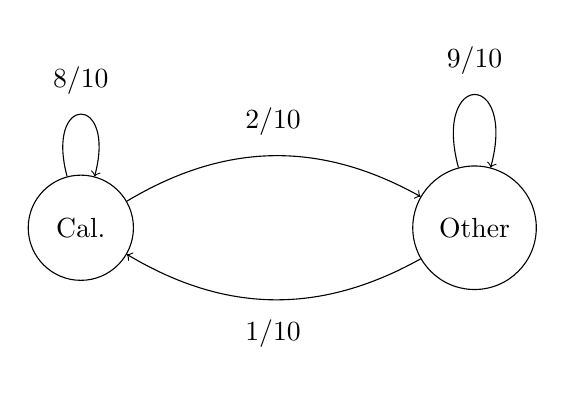
\begin{tikzpicture}[inner sep=7pt]
        \node[circle, draw] (A) at (0,0) {Cal.};
        \node[circle, draw] (B) at (5,0) {Other};

        \draw[->] (A) to[bend left] node[above] {2/10} (B);
        \draw[->] (B) to[bend left] node[below] {1/10} (A);

        \draw[->] (A) to[loop above] node {8/10} (A);
        \draw[->] (B) to[loop above] node {9/10} (B);
    \end{tikzpicture}
    \caption{Markov Process}
\end{figure}

The essential assumption of Markov process is
\begin{itemize}
    \item The population in both states is constant and never be negative.
    \item The $u_{k+1}$ only depends on $u_k$ i.e. \[
        u_{k+1} = A u_k
    \]
    \item The total population is constant.
    \begin{enumerate}
        \item all entries are positive or zero.
        \item column sums are 1.
    \end{enumerate}
\end{itemize}

\newpage

\begin{eg}
    \[
        A = \begin{pmatrix}
            9/10 & 2/10 \\
            1/10 & 8/10
        \end{pmatrix}
    \]
\end{eg}

We have \[
    \det(A - \lambda I) = \lambda^2 - \frac{17}{10}\lambda + 1 = 0 \implies \lambda_1 = 1, \lambda_2 = \frac{7}{10}
\]
Since \[
    A = \begin{pmatrix}
        2/3 & 1/3 \\
        1/3 & -1/3
    \end{pmatrix} \begin{pmatrix}
        1 & 0 \\
        0 & 7/10
    \end{pmatrix} \begin{pmatrix}
        1 & 1 \\
        1 & -2
    \end{pmatrix} \quad (A = S \Lambda S^{-1})
\]
We have \begin{align*}
    \begin{pmatrix}
        y_k \\ z_k
    \end{pmatrix} &= A^k \begin{pmatrix}
        y_0 \\ z_0
    \end{pmatrix} = \begin{pmatrix}
        2/3 & 1/3 \\
        1/3 & -1/3
    \end{pmatrix} \begin{pmatrix}
        1^{\red{k}} & 0 \\
        0 & (7/10)^{\red{k}}
    \end{pmatrix} \begin{pmatrix}
        1 & 1 \\
        1 & -2
    \end{pmatrix} \begin{pmatrix}
        y_0 \\ z_0
    \end{pmatrix} \qquad \blue{ c = \begin{pmatrix}
        y_0 + z_0 \\ y_0 - 2z_0
    \end{pmatrix} } \\[6pt]
    &= (y_0 + z_0) (1)^k \cdot \begin{pmatrix}
        2/3 \\ 1/3
    \end{pmatrix} + (y_0 - 2z_0) (7/10)^k \cdot \begin{pmatrix}
        1/3 \\ -1/3
    \end{pmatrix}
\end{align*}

When $k \to \infty$, we have \[
    \lim_{k \to \infty} \begin{pmatrix}
        y_k \\ z_k
    \end{pmatrix} = (y_0 + z_0) \begin{pmatrix}
        2/3 \\ 1/3
    \end{pmatrix}
\]
i.e. No matter what the initial population distribution is, the population will eventually stabilize at 2/3 outside and 1/3 inside.
\[
    \begin{pmatrix}
        0.9 & 0.2 \\
        0.1 & 0.8
    \end{pmatrix} \begin{pmatrix}
        2/3 \\ 1/3
    \end{pmatrix} = \begin{pmatrix}
        2/3 \\ 1/3
    \end{pmatrix} \quad \text{ or } \quad A u_{\infty} = u_{\infty}
\]
The \textbf{steady state} $u_{\infty}$ is an eigenvector of $A$ corresponding to $\lambda = 1$.